\documentclass{standalone}

\usepackage{animate}
\usepackage{amsmath, amssymb, amsthm, mathrsfs, amsfonts, dsfont}
\usepackage{ascmac}
\usepackage{bbm}
\usepackage{bm}
\usepackage{breakcites}
\usepackage{calc}
\usepackage{enumerate}
\usepackage{ifthen}
\usepackage{mathtools}
\usepackage{makecell}
\usepackage{mlmodern}
\usepackage{newtxtext}
\usepackage{optidef}
\usepackage{physics}
\usepackage{pifont}
\usepackage{setspace}
\usepackage{stfloats}
\usepackage{subcaption}
\usepackage{svg}
\usepackage{tikz}
\usepackage{xparse}
\usepackage[all]{xy}

\usepackage{float}
\usepackage{color}
\usepackage{graphicx}
\usepackage[colorlinks=true, allcolors=blue]{hyperref}


% === Commands ===

\definecolor{cA}{HTML}{0072BD}
\definecolor{cB}{HTML}{EDB120}
\definecolor{cC}{HTML}{77AC30}
\definecolor{cD}{HTML}{D95319}
\definecolor{cE}{HTML}{7E2F8E}
\newcommand{\cAText}[1]{\textcolor{cA}{#1}}
\newcommand{\cBText}[1]{\textcolor{cB}{#1}}
\newcommand{\cCText}[1]{\textcolor{cC}{#1}}
\newcommand{\cDText}[1]{\textcolor{cD}{#1}}
\newcommand{\cEText}[1]{\textcolor{cE}{#1}}
\newcommand{\red}[1]{\textcolor{red}{#1}}
\newcommand{\blue}[1]{\textcolor{blue}{#1}}
\newcommand{\green}[1]{\textcolor{green}{#1}}
\newcommand{\gray}[1]{\textcolor{gray}{#1}}
\newcommand{\black}[1]{\textcolor{black}{#1}}

\newcommand{\st}{\text{ s.t. }}
\newcommand{\Img}[1]{\mathrm{Im}\qty(#1)}
\newcommand{\Ker}[1]{\mathrm{Ker}\qty(#1)}
\newcommand{\Supp}[1]{\mathrm{supp}\qty(#1)}
\newcommand{\Rank}[1]{\mathrm{rank}\qty(#1)}
\newcommand{\floor}[1]{\left\lfloor #1 \right\rfloor}
\newcommand{\ceil}[1]{\left\lceil #1 \right\rceil}
% C++ (https://tex.stackexchange.com/questions/4302/prettiest-way-to-typeset-c-cplusplus)
\newcommand{\Cpp}{C\nolinebreak[4]\hspace{-.05em}\raisebox{.4ex}{\relsize{-3}{\textbf{++}}}}
% https://tex.stackexchange.com/questions/28836/typesetting-the-define-equals-symbol
\newcommand{\defeq}{\coloneqq}
\newcommand{\eqdef}{\eqqcolon}
% https://tex.stackexchange.com/questions/5502/how-to-get-a-mid-binary-relation-that-grows
\newcommand{\relmiddle}[1]{\mathrel{}\middle#1\mathrel{}}
\newcommand{\cmark}{\cCText{\ding{51}}} % check mark
\newcommand{\xmark}{\cDText{\ding{55}}} % cross mark

\DeclareMathOperator{\Proj}{Proj}
\DeclareMathOperator{\Exp}{Exp}
\DeclareMathOperator{\Hess}{Hess}
\DeclareMathOperator{\Retr}{Retr}
\DeclareMathOperator{\Span}{span}
\DeclareMathOperator{\myGrad}{grad}
\renewcommand{\grad}{\myGrad}

% https://tex.stackexchange.com/questions/564216/newcommand-for-each-letter
\ExplSyntaxOn
\NewDocumentCommand{\definealphabet}{mmmm}{
\int_step_inline:nnn{`#3}{`#4}{
\cs_new_protected:cpx{#1 \char_generate:nn{##1}{11}}{
\exp_not:N #2{\char_generate:nn{##1}{11}}}}}
\ExplSyntaxOff

\definealphabet{bb}{\mathbb}{A}{Z}
\definealphabet{rm}{\mathrm}{A}{Z}
\definealphabet{cal}{\mathcal}{A}{Z}
% \definealphabet{scr}{\mathscr}{A}{Z}
\definealphabet{frak}{\mathfrak}{a}{z}
\definealphabet{frak}{\mathfrak}{A}{Z}

% === Settings ===

% https://qiita.com/rityo_masu/items/efd44bc8f9229e014237
\allowdisplaybreaks[4]

\usetikzlibrary{
  3d,
  fit,
  calc,
  math,
  shapes,
  matrix,
  patterns,
  backgrounds,
  arrows.meta,
  decorations.pathmorphing,
}

\begin{document}

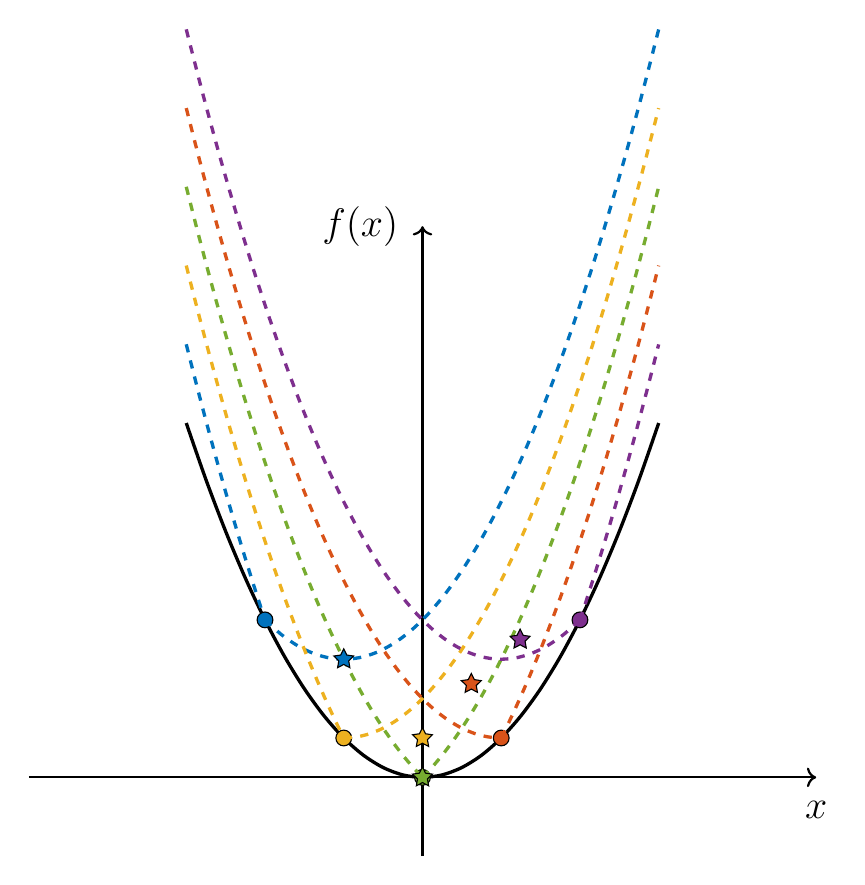
\begin{tikzpicture}
    \draw[->,thick] (-5,0) -- (5,0) node[below=0.5em] {\Large$x$};
    \draw[->,thick] (0,-1) -- (0,7) node[left=0.5em] {\Large$f(x)$};

    \draw[domain=-3:3, smooth, variable=\x, very thick] plot ({\x}, {0.5*\x*\x});

    \foreach \v/\c in {-2/cA,-1/cB,0/cC,1/cD,2/cE} {
            \draw[fill=\c] (\v,{0.5*(\v)^2}) circle (0.1);

            % draw 0.5*(x-v)^2+|x|
            \ifnum \v=-2
                \draw[\c, domain=-3:-2, smooth, variable=\x, dashed, very thick] plot ({\x}, {0.5*(\x)^2 + \v - \x});
                \draw[\c, domain=-2:+3, smooth, variable=\x, dashed, very thick] plot ({\x}, {0.5*(\x)^2 - \v + \x});
            \fi
            \ifnum \v=-1
                \draw[\c, domain=-3:-1, smooth, variable=\x, dashed, very thick] plot ({\x}, {0.5*(\x)^2 + \v - \x});
                \draw[\c, domain=-1:+3, smooth, variable=\x, dashed, very thick] plot ({\x}, {0.5*(\x)^2 - \v + \x});
            \fi
            \ifnum \v=0
                \draw[\c, domain=-3:+0, smooth, variable=\x, dashed, very thick] plot ({\x}, {0.5*(\x)^2 + \v - \x});
                \draw[\c, domain=+0:+3, smooth, variable=\x, dashed, very thick] plot ({\x}, {0.5*(\x)^2 - \v + \x});
            \fi
            \ifnum \v=1
                \draw[\c, domain=-3:+1, smooth, variable=\x, dashed, very thick] plot ({\x}, {0.5*(\x)^2 + \v - \x});
                \draw[\c, domain=+1:+3, smooth, variable=\x, dashed, very thick] plot ({\x}, {0.5*(\x)^2 - \v + \x});
            \fi
            \ifnum \v=2
                \draw[\c, domain=-3:+2, smooth, variable=\x, dashed, very thick] plot ({\x}, {0.5*(\x)^2 + \v - \x});
                \draw[\c, domain=+2:+3, smooth, variable=\x, dashed, very thick] plot ({\x}, {0.5*(\x)^2 - \v + \x});
            \fi
        }

    \foreach \v/\c in {-2/cA,-1/cB,0/cC,1/cD,2/cE} {
            \ifnum \v=-2
                \node[star, star point height=0.05cm, star point ratio=2.0, scale=0.4, draw=black, fill=\c] at (-1,1.5) {};
            \fi
            \ifnum \v=-1
                \node[star, star point height=0.05cm, star point ratio=2.0, scale=0.4, draw=black, fill=\c] at (0,0.5) {};
            \fi
            \ifnum \v=0
                \node[star, star point height=0.05cm, star point ratio=2.0, scale=0.4, draw=black, fill=\c] at (0,0) {};
            \fi
            \ifnum \v=1
                \node[star, star point height=0.05cm, star point ratio=2.0, scale=0.4, draw=black, fill=\c] at (0.62,1.18752) {};
            \fi
            \ifnum \v=2
                \node[star, star point height=0.05cm, star point ratio=2.0, scale=0.4, draw=black, fill=\c] at (1.24,1.75) {};
            \fi
        }
\end{tikzpicture}

\end{document}